\begin{figure*}[tb]
\centerline{
\includegraphics[width=2.8in, angle=270 ]{./figures/GrabSeq.eps}
} \caption{Grasping behavior: an example. Sequence of the robot 
grasping a porcelain cup. Frame 1: the cup is presented to the 
robot. Frame 2: the robot reaches for the cup. Frames 3 to 6:  
the robot explores the
space and uses tactile feedback to find the object and adjust the
position of the hand. Frames 7 and 8: the robot grasps 
and lifts the cup.} \label{fig:sequence}
\end{figure*}

\section{Results}
\label{sec:results}

\begin{table*}[htb]
  \caption{Objects.} \label{tab:objects} \centering
  \begin{tabular}{|c|l|c|c|c|l|}
    \hline
    &Description& Weight(Kg)&No.Trials&No.Failures&Contains \\
    %&Object& W(Kg)&Trials&Fail&Contains \\
    \hline
    1&Plastic bottle        & 0.265 & 22& 0 & Vitamins\\
    2&Porcelain cup & 0.255 & 24& 1 & Nothing\\
    3&Plastic cup (Starbucks)      & 0.220 & 24& 4 & Bolts \\
    4&Rectangular box (Nesquick)        & 0.240 & 34& 2 & Nesquick powder\\

    \hline
  \end{tabular}
\end{table*}

\begin{figure*}[tbp]
\centerline{
\includegraphics[width=6.0in]{./figures/objects-clusters3.eps}
}\caption{Right: the set of objects used in the experiments: a plastic bottle,
a porcelain cup, a plastic cup and a rectangular plastic box. Some objects were
partially filled to increase the weight (all objects weighed about 220-250g).
Left: visualization of the clusters. The grid plots the winning units for each object. To better quantify the separation of the clusters in feature space we report the unified unit matrix representation (U-matrix) of the SOM. This representation codes the distance between neighboring units (dark and light areas represent units whose weights are very close or very far to each others, respectively). In the U-matrix clusters are formed by dark areas separated by light regions. In our case only three clusters are formed: the two cups are not clearly separated because have similar shape.}
\label{fig:Objects}
\end{figure*}

%% \begin{figure}[tbp]
%% \centerline{
%% 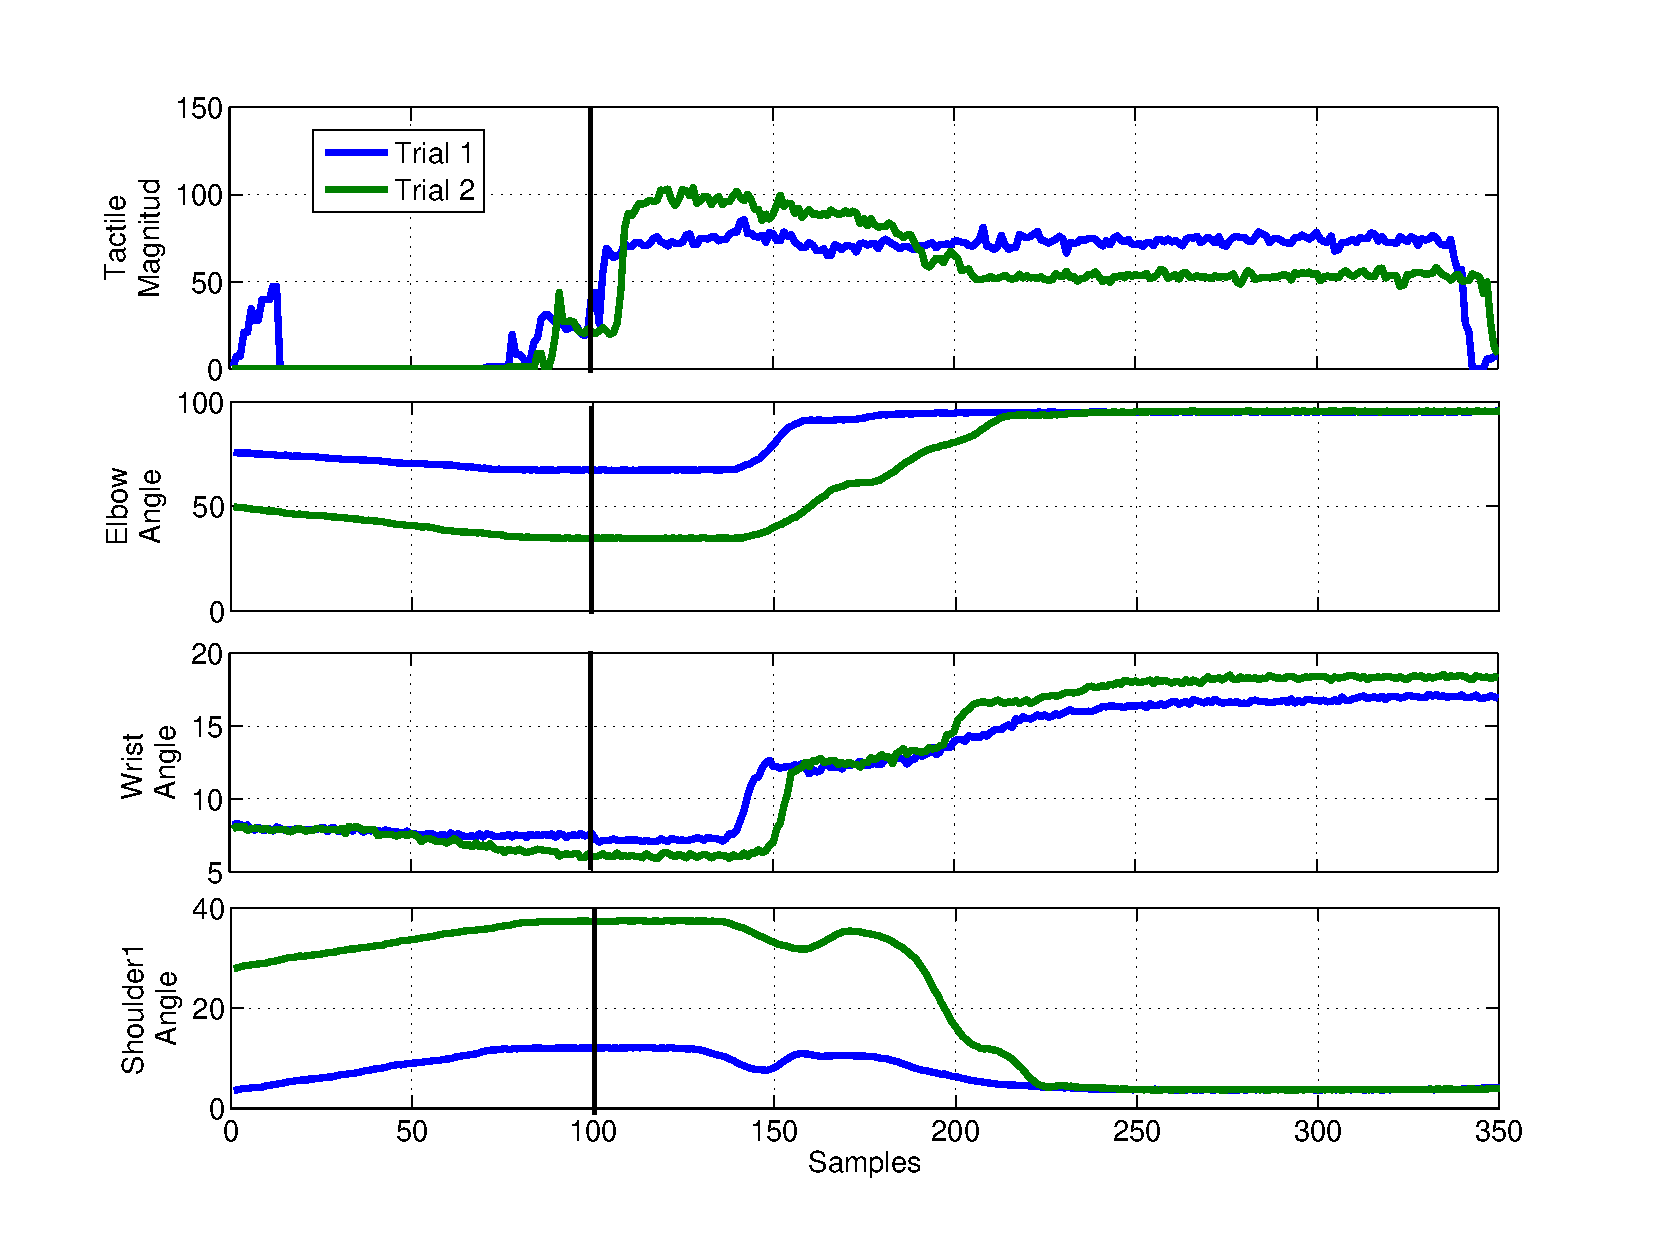
\includegraphics[width=3.5in]{./figures/GraspingData1.eps}
%% }\caption{The figure presents the trajectories followed by two
%% different grasping sequences of a same object. We can observe that
%% the tactile sensor response capture the variation in the different
%% trajectories. The magnitude of the tactile vector is the vectorial
%% summation of the forces present in each tactile sensor considering
%% the current geometry of the hand.} \label{fig:AnglesPlot}
%% \end{figure}

%% \begin{figure}[tbp]
%% \centerline{
%% 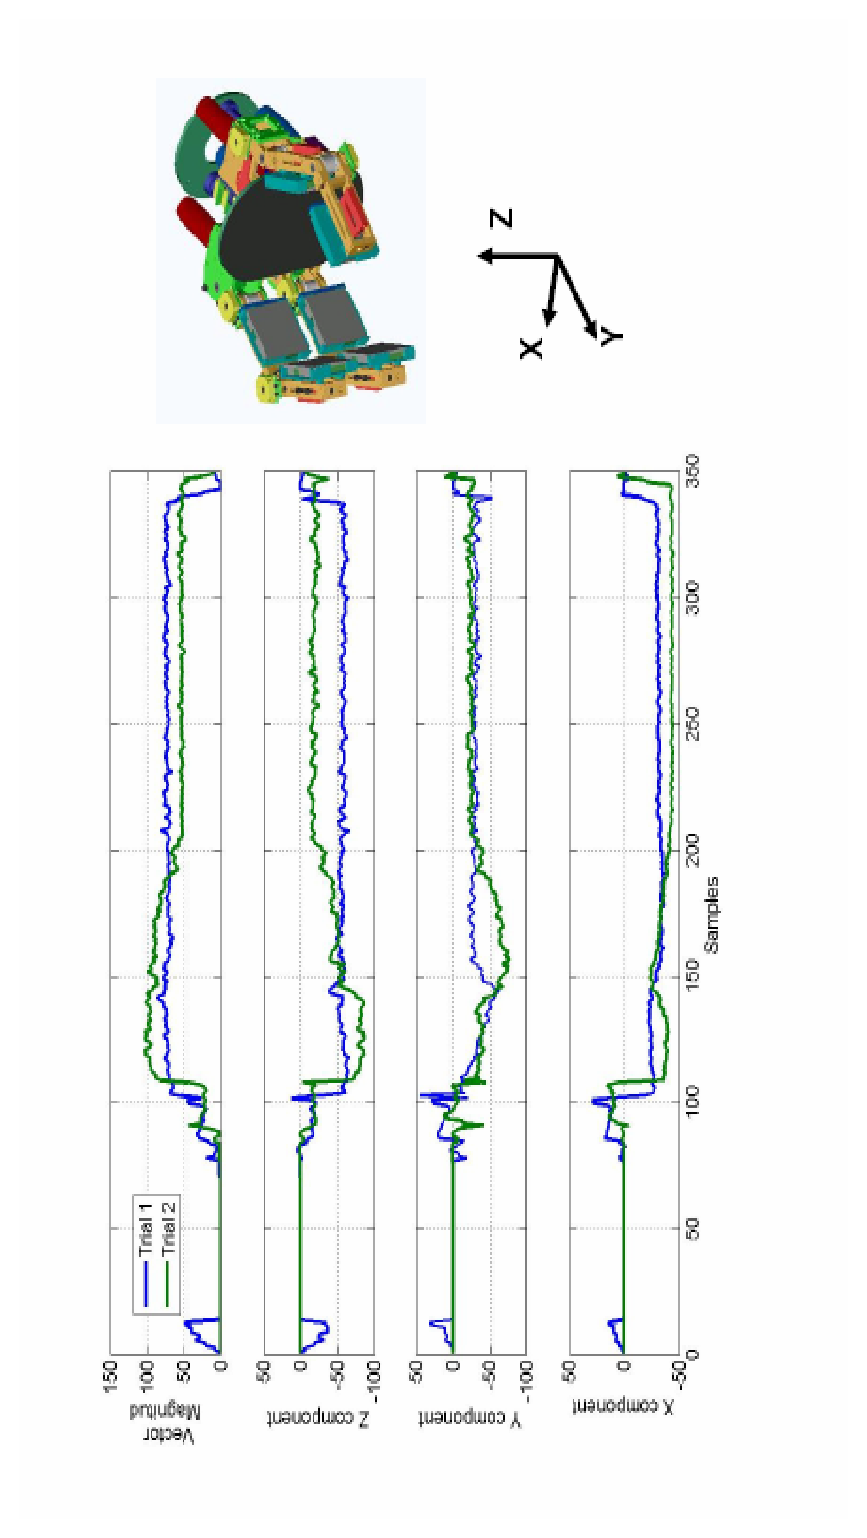
\includegraphics[height=3.2in, angle=270]{./figures/TactileComp.eps}
%% }\caption{The magnitude of the tactile vector is the vectorial
%% summation of the forces present in each tactile sensor considering
%% the current geometry of the hand.} \label{fig:TactileComp}
%% \end{figure}

The grasping behavior described in Section~\ref{sec:controlling}
was evaluated by presenting different objects to the robot and by
counting the number of successful grasps. We chose objects of
different size and shape: a plastic bottle, a plastic rectangular
box, a porcelain cup and a plastic cup (see
figure~\ref{fig:Objects}). Some of the objects were partially
filled, so that the weight was roughly uniform among all objects
(about 220-250 grams, see Table~\ref{tab:objects}). The robot had 
no prior knowledge about these objects. 

Each object was presented to the robot several times and 
randomly placed on the table. Overall the number of grasping
trials was 104, of which only 7 were not successful. In some of
these trials, the robot managed to grasp the object, but was not
able to hold it because the grip did not produce enough friction.
In a few cases the tactile sensors failed to detect the object and
the exploration was aborted before the object was actually
grasped (more details are reported in Table~\ref{tab:objects}).

As a further validation, we clustered the haptic information
originated from the grasping. We collected the hand feedback at
the moment the robot lifted the object; the idea is that given the
intrinsic compliance of the hand, its configuration and the force
exerted by each joint depend on the shape of the object being
grasped. Given the high dimensionality of the problem we used
a Self Organizing Map (SOM) to visualize and plot the data collected
during the experiment (at this purpose we employed the SOM toolbox for 
Matlab \cite{somToolbox}).
%the data collected during the experiment is difficult (plotting
%a subset of them does not seem significant either). To analyze this
%data we clustered it by means of a Self Organizing Map (SOM). 
The SOM clusters the input data so that similar vectors activate 
nearby neurons.
The results show that the bottle, the rectangular box and the cups 
form three clusters (see figure~\ref{fig:Objects}). 
Unfortunately the clusters formed by the two cups are not clearly
distinguishable. This is probably due to the fact that the hand
grasped the objects from the top, where the two
objects are quite alike (both are circular with similar diameter).
In these cases the limited number of fingers (three) made it hard
to distinguish between the cylindrical and conic shape of the
cups. 

Together the results prove that the grasping behavior of the
robot is reliable and that allows gathering data that could 
potentially used for learning. The high number of successful trials shows that
the haptic feedback manages to drive the robot during the
exploration until it finds the object and grasps it. This is
further demonstrated by the clustering. The fact that during 
different trials the same object activates nearby units 
shows that the grasping behavior produces similar grasps.

% and that 
%the data gathered by the robot carries meaningful 
%information about the physical shape of the objects.

It is finally worth commenting on the objects we have used in this experiment. 
Although different the objects
have somewhat similar size and elongated shape. It is fair to say that 
the robot would fail to grasp objects of much smaller or bigger 
size or having more complex shapes. This limitation is in part due to 
the size of the hand that does not allow gripping very 
small objects or part of them (like a screw or the handle of a cup). 
It is also true, on the other hand, that the grasping behavior we have
described is still quite simple and needs to be improved to cope with 
more challenging situations (for example by allowing the hand to approach
the objects from above and with different orientations).
%
%The data gathered by the robot carries meaningful information about
%the physical shape of the objects and could potentially be used to
%train a classifier.
%which show that the
%behavior allows extracting meaningful information about the
%physical properties of the objects (i.e. their shape).
